\section{Database View}

This section contains definitions of data and information structures that have to be implemented in the database.

\subsection{Data4Help}

In \textbf{picture \ref{fig:D4H-er}} there is the ER diagram for the D4H database.
There are four main entities:
\begin{itemize}
    \item \textbf{User}: used to store D4H user information, it is inherited by Individual and Third-party entities.
    \item \textbf{Health data}: used to store data gathered through the smart-watch, it is associated to exactly one individual and it is characterised by time stamp (date and time), position (latitude and longitude) and health data (BPM, Daily steps). 
    \item \textbf{Subscription}: used to store requests with Subscription; it's associated to the Third-party that made the request, to the Individual that the Third-party is asking for and to the particular health data record.
    \item \textbf{Request}: used to store a request for health data and the Third-Party who made the request; can be either Single (requesting a single health data record) or Multiple (requesting multiple health data records).
\end{itemize}

\begin{figure}[H]
    \centering
    \makebox[\textwidth][c]{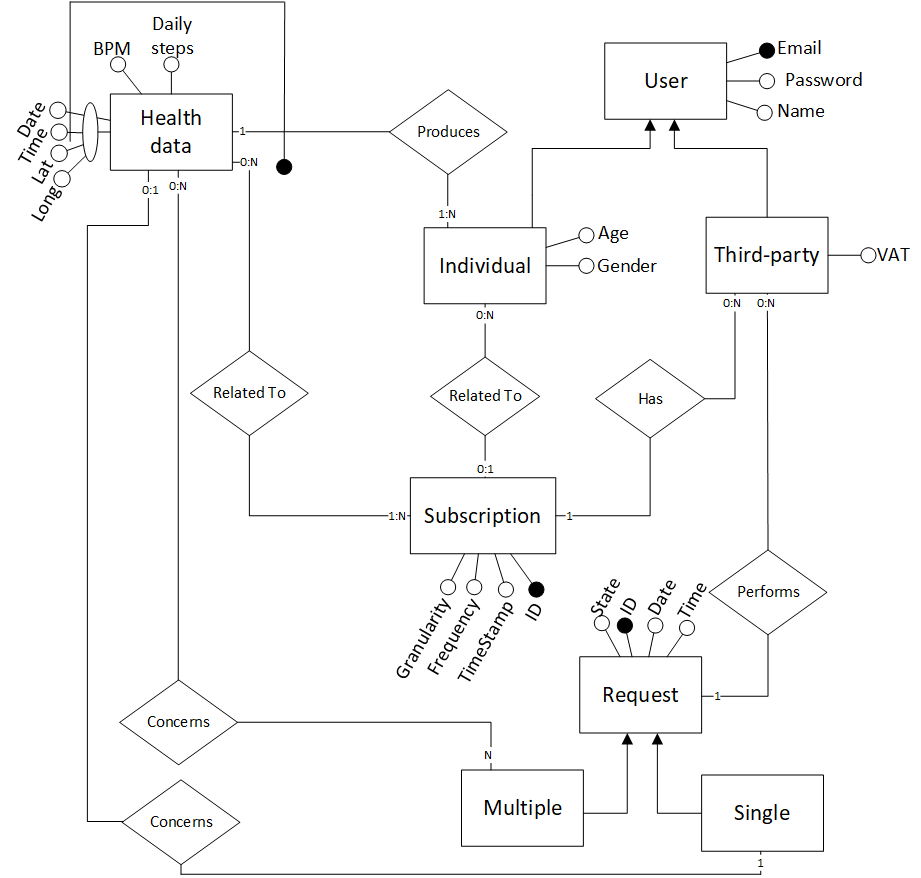
\includegraphics[scale=0.70]{pictures/D4H_ER.png}}
    \caption{D4H database ER diagram}
    \label{fig:D4H-er}
\end{figure}

In the picture below (\textbf{picture \ref{fig:D4H-Logic-Schema}}) there is the the conversion from the ER diagram described before to a Logic Schema.

\begin{figure}[H]
    \centering
    \makebox[\textwidth][c]{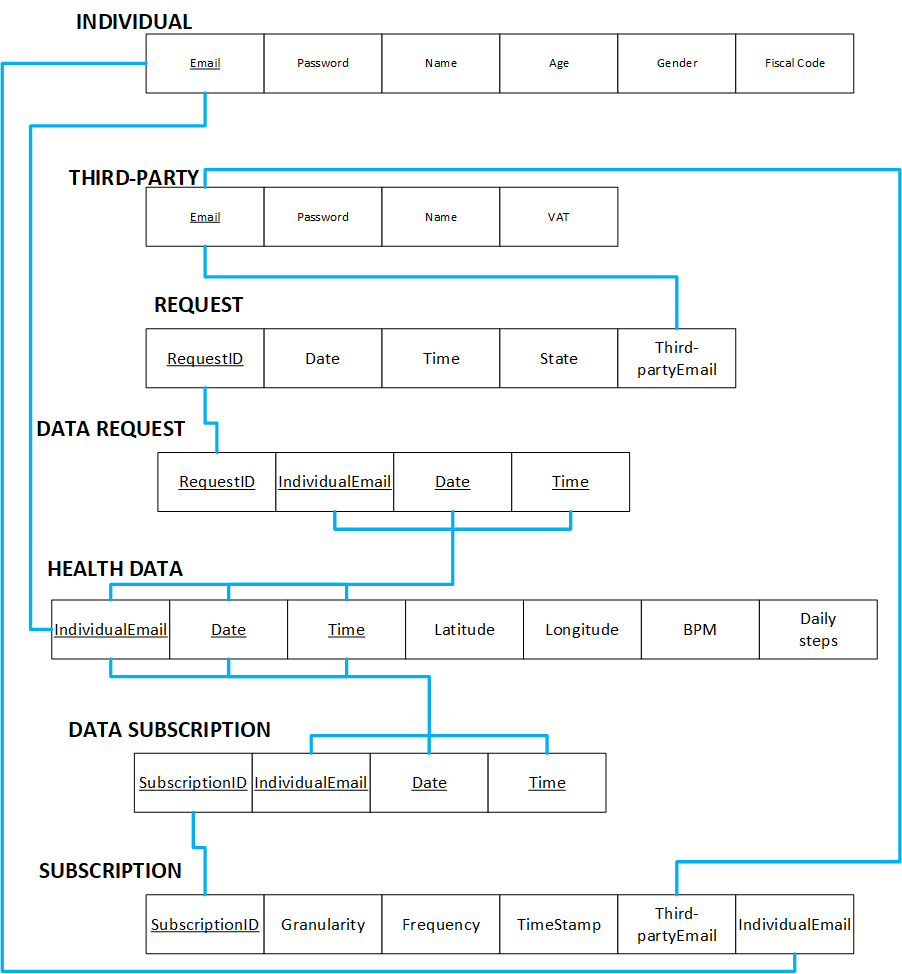
\includegraphics[scale=0.65]{pictures/D4H_Logic_Schema.png}}
    \caption{D4H Logic Schema}
    \label{fig:D4H-Logic-Schema}
\end{figure}


\subsection{Track4Run}

\textbf{Figure \ref{fig:T4R-er}} represents the ER diagram of the T4R system. Track4Run needs to store data related to Organiser and Participant accounts and information about races.

In this case, he main entities are:
\begin{itemize}
    \item \textbf{Organiser}: it models Organiser account data such as its name, email, password, etc. An organiser can organise zero, one or more races.
    \item \textbf{Participant}: this entity is used to store Participant account information. It is associated to \emph{Race} through the ``enrols" relation.
    \item \textbf{Race}: this is the entity containing race details, such as the ID, the location, date and time; there is a relation between \emph{Race} and \emph{Organiser}.
    \item \textbf{Ranking}: it is used to store participants' arrival rankings in past races. Any Participant can be involved in one or more rankings if he enrolled in one or more races in the past.
    \item \textbf{Path}: Every race tuple is associated to a path; it is represented by a starting point, an ending point, a total length and n middle positions between the starting and the ending locations. A single path can be associated to more then one race.
\end{itemize}

\begin{figure}[H]
    \centering
    \makebox[\textwidth][c]{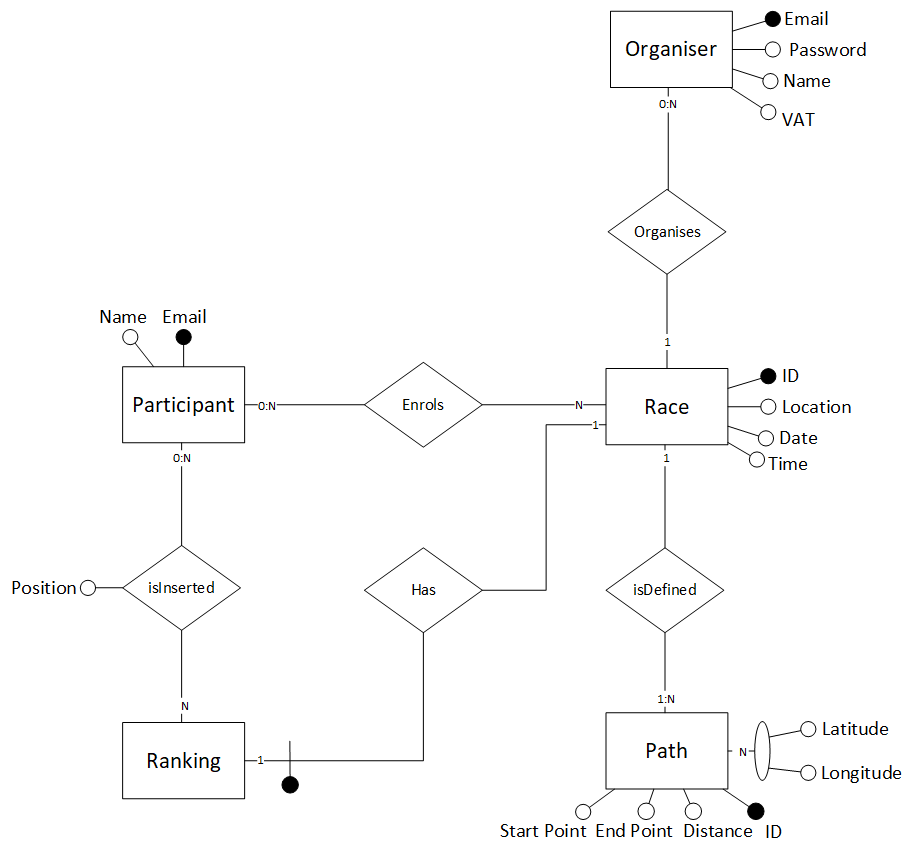
\includegraphics[scale=0.70]{pictures/T4R_ER.png}}
    \caption{T4R database ER diagram}
    \label{fig:T4R-er}
\end{figure}

As already done for D4H, also for T4R we show the ER diagram conversion to Logic Schema (\textbf{figure \ref{fig:T4R-Logic-Schema}}).

\begin{figure}[H]
    \centering
    \makebox[\textwidth][c]{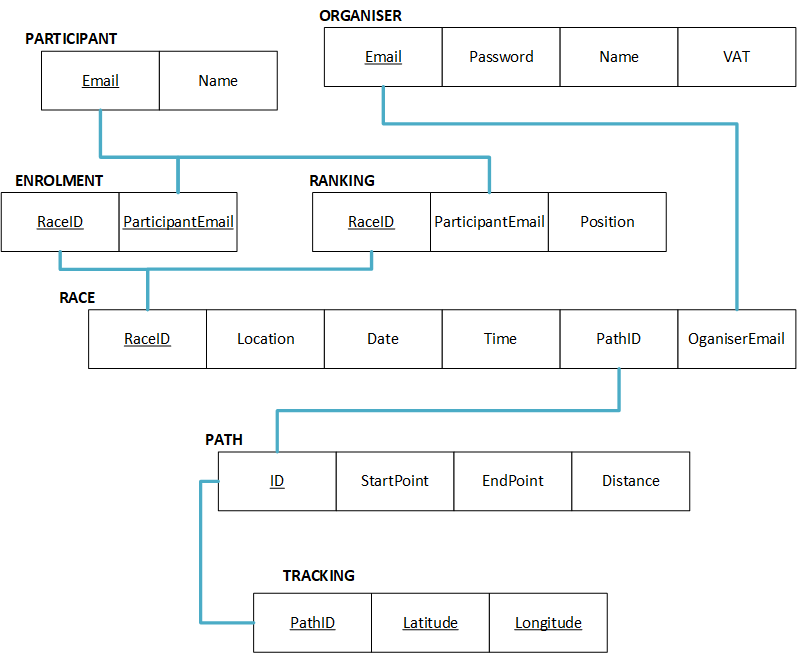
\includegraphics[scale=0.70]{pictures/T4R_Logic_Schema.png}}
    \caption{T4R Logic Schema}
    \label{fig:T4R-Logic-Schema}
\end{figure}